\itemhead{习题3.2 · 第5题（教材p.85）}{XJ-B1-C03-HW-P085-Y1280}
\label{XJ-B1-C03-HW-P085-Y1280}
{\footnotesize 湘教版教材p.85 / PDF第92页 / 习题3.2 / 第5题}
\field{原题}{已知 $f(x)$ 与 $g(x)$ 分别是定义在 $\mathbb R$ 上的偶函数和奇函数，将下图补充完整。
\bankfig{C03-HW085-05}{0.85}}
\field{参考答案}{将 $f$ 已知图象上的每个点 $(x,y)$ 映为 $(-x,y)$ 补另一侧；将 $g$ 上每个点映为 $(-x,-y)$。原有空、实端点随对称一起保留；若0属于奇函数定义域，图象必须过原点。}
\begin{center}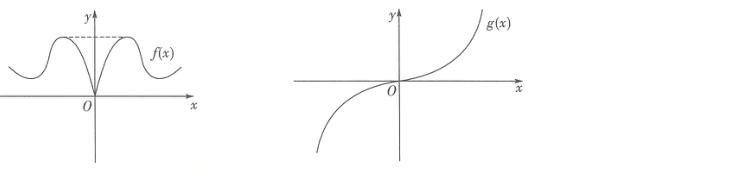
\includegraphics[width=.84\linewidth,height=.38\textheight,keepaspectratio]{figures/C03-HW085-5-source.png}\end{center}
{\footnotesize 补图来源：所给答案册PDF第24页（册内23页），已核对对应关系。}\par
{\small \field{关联知识}{F08 奇偶性、对称与函数性质应用（教材帮p.113、114、115 / PDF122、123、124）；F04 函数三种表示法、图象与读数（教材帮p.85、86、93、94 / PDF94、95、102、103）}
\field{方法与易错点}{检查定义域，再代入 $-x$；求另一侧解析式时同时写出 $-x$ 所在区间。 易错：只看公式不看定义域；用一对点证明奇偶；负半轴代换遗漏最外层负号。}
\field{答案依据}{答案册相关题组：PDF第23、24页（册内页22、23）；按当前题库原题逐项重算，不按旧版题号机械对套。}}
